\section{Lösungsstrategie}
\label{sec:loesungsstrategie}

Dieses Kapitel beschreibt die grundlegenden Architekturentscheidungen
und Lösungsansätze. Detaillierte Begründungen finden sich in den ADRs
(Kap.~9).

\subsection{Kernarchitekturentscheidung}
\label{sec:kernarchitekturentscheidung}

EduPlanner folgt einer
\textbf{Microservice-Architektur}\footnotemark{},
ausgerichtet an den fünf fachlichen
Bounded~Contexts\footnotemark{}
aus dem Domain-Driven Design (DDD).
Jeder Bounded Context wird als eigenständiger Dienst mit eigener
Datenbank (Database-per-Service-Pattern) implementiert.
$\to$ Vollständige Begründung: ADR-001.

\addtocounter{footnote}{-2}
\stepcounter{footnote}
\footnotetext{%
  \textbf{Microservice-Architektur.}
  Ein Architekturstil, bei dem eine Anwendung als Sammlung kleiner,
  eigenständiger Dienste (\emph{Services}) realisiert wird. Jeder
  Service ist unabhängig deploybar, besitzt einen eigenen
  Datenhaushalt und kommuniziert mit anderen Services über
  wohldefinierte Schnittstellen (typischerweise REST oder
  asynchrone Nachrichten). Im Gegensatz zum monolithischen Ansatz
  lassen sich einzelne Services unabhängig skalieren, aktualisieren
  und durch verschiedene Teams weiterentwickeln.
  Vgl.\ Sam Newman, \emph{Building Microservices}, O'Reilly, 2021.%
}

\stepcounter{footnote}
\footnotetext{%
  \textbf{Bounded Context (Domain-Driven Design).}
  Ein \emph{Bounded Context} ist ein zentrales Konzept aus dem
  Domain-Driven Design (DDD) von Eric Evans. Er definiert eine
  explizite Grenze, innerhalb derer ein bestimmtes Domänenmodell
  mit einer einheitlichen Fachsprache (\emph{Ubiquitous Language})
  gilt. Ausserhalb dieser Grenze können dieselben Begriffe eine
  andere Bedeutung haben -- z.\,B.\ meint ``Kurs'' im Context
  \texttt{catalog} die inhaltliche Beschreibung, im Context
  \texttt{scheduling} hingegen eine konkrete Durchführung mit
  Datum und Ort.
  Bounded Contexts bilden in einer Microservice-Architektur die
  natürlichen Dienstgrenzen: ein Service pro Bounded Context.
  Vgl.\ Eric Evans, \emph{Domain-Driven Design}, Addison-Wesley,
  2003.%
}

\subsubsection{Microservices vs. Modularer Monolith -- Faire Gegenüberstellung}

\begin{reviewbox}[Didaktische Anmerkung]
Die Entscheidung für Microservices ist bei kleinem Team und engem MVP-Scope nicht
selbstverständlich. Nachfolgend eine explizite Gegenüberstellung beider Optionen --
denn für EduPlanner wäre ein modularer Monolith zunächst die \emph{einfachere}
Wahl gewesen.
\end{reviewbox}

\begin{tabularx}{\textwidth}{L{4cm} X X}
  \rowcolor{tableheader}
  \color{white}\textbf{Kriterium} &
  \color{white}\textbf{Modularer Monolith} &
  \color{white}\textbf{Microservices (gewählt)} \\
  Betriebskomplexität &
  Gering: 1~Prozess, 1~Datenbank, 1~Deployment-Artefakt. &
  Hoch: 5~Services, 5~Datenbanken, Message Broker, API Gateway. \\
  \rowcolor{tablegrey}
  Lokale Entwicklung &
  Einfach: \texttt{mvn spring-boot:run} genügt. &
  Aufwändig: Docker Compose mit 8+ Containern. \\
  Skalierbarkeit &
  Immer das gesamte System; keine Teilskalierung. &
  Selektiv: \texttt{registration} zur Spitzenzeit auf 10~Pods,
  \texttt{catalog} auf 1~Pod. \\
  \rowcolor{tablegrey}
  Team-Autonomie &
  Gemeinsames Codebase; Merge-Konflikte bei paralleler Entwicklung. &
  Separate Repositories; Teams deployen unabhängig. \\
  Datenkonsistenz &
  ACID-Transaktionen über Modulgrenzen hinweg. &
  Nur Eventual Consistency; Saga-Muster für verteilte Transaktionen. \\
  \rowcolor{tablegrey}
  Einstiegshürde &
  Niedrig: Standard-Wissen reicht. &
  Hoch: Verteilte Systeme, Netzwerkpartitionen, Observability. \\
  Technische Schulden &
  Modulgrenzen erodieren mit der Zeit (``Big Ball of Mud''). &
  Service-Grenzen sind hart; Erosion schwerer möglich. \\
  \rowcolor{tablegrey}
  Passt für EduPlanner? &
  Ja -- für MVP und kleine Teamgrösse sogar naheliegender. &
  Ja -- wenn Skalierbarkeit und Team-Autonomie langfristig wichtiger
  sind als kurzfristige Einfachheit. \\
\end{tabularx}

\begin{hinweis}[Warum trotzdem Microservices?]
Drei konkrete Faktoren haben den Ausschlag gegeben
(vollständige Begründung in ADR-001):
\begin{enumerate}[leftmargin=2em]
  \item \textbf{Unterschiedliche Skalierungsbedarfe:} Der
  \texttt{registration}-Service muss zur Einschreibungsfrist horizontal
  skalieren; \texttt{catalog} und \texttt{notification} haben einen
  Bruchteil der Last. Im Monolithen wäre nur vertikale Skalierung des
  Gesamtsystems möglich.
  \item \textbf{Klare fachliche Grenzen:} Die fünf Bounded Contexts haben
  grundlegend verschiedene Änderungsraten (Katalog ändert sich selten,
  Einschreibungslogik häufig). Getrennte Deployments vermeiden, dass ein
  stabiles Modul wegen Änderungen an einem anderen neu deployt wird.
  \item \textbf{Lernziel der Unterrichtsunterlage:} Microservices sind
  in der Praxis weit verbreitet; die Dokumentation zeigt Studierenden
  ein realistisches Architekturmuster mit seinen echten Trade-offs
  (vgl.\ ATAM-light, Kap.~10.1).
\end{enumerate}
\textbf{Modularer Monolith als Fallback:} Falls der Betriebsaufwand das
Team überfordert, ist ein Rückbau auf einen modularen Monolithen explizit
als Risikomitigierung geplant (Risiko R5, Kap.~11).
\end{hinweis}

% ──────────────────────────────────────────────
\subsection{Fachliche Strategie (Domain-Driven Design)}

\begin{enumerate}[leftmargin=2em]

  \item \textbf{Event~Storming} (nach Alberto Brandolini) als
  kollaborative Methode zur Domänenentdeckung.
  Dabei modellieren Fachexperten und Entwickler gemeinsam
  mit Hilfe eines Whiteboards den gesamten Geschäftsprozess -- ausgehend
  von \emph{Ereignissen} (``Teilnehmer hat sich
  eingeschrieben'', ``Kurs wurde veröffentlicht'' etc.).
  Aus den entdeckten Ereignissen lassen sich natürliche
  fachliche Grenzen ableiten, die direkt in die
  Bounded-Context-Struktur einfliessen.
  Das Event-Storming-Ergebnis für EduPlanner ist in
  Anhang~A dokumentiert.

  \item \textbf{5~Bounded Contexts} als natürliche Dienstgrenzen.
  EduPlanner definiert fünf Kontexte mit klarer fachlicher
  Verantwortlichkeit: \texttt{catalog},
  \texttt{scheduling}, \texttt{registration},
  \texttt{notification} und \texttt{identity}.
  Die Kontextgrenzen wurden im Event Storming identifiziert
  und decken sich bewusst 1:1 mit den Servicegrenzen
  (Details siehe Abschnitt~4.2.1).

  \item \textbf{Ubiquitous Language} (allgegenwärtige Sprache)
  je Kontext. Jeder Bounded Context pflegt ein eigenes,
  verbindliches Vokabular, das sowohl im Fachgespräch als
  auch im Quellcode (Klassen, Methoden, Events) konsistent
  verwendet wird. Dadurch wird sichergestellt, dass
  Missverständnisse zwischen Fachseite und Entwicklung
  minimiert werden. Das vollständige Glossar pro Context
  findet sich in Kap.~12.

  \item \textbf{Domain Events} als primäres Muster der
  kontextübergreifenden Kommunikation.
  Wenn in einem Bounded Context ein fachlich relevantes
  Ereignis eintritt (z.\,B.\
  \texttt{EnrollmentConfirmed}), wird dieses als
  \emph{Domain Event} über den Message Broker
  (RabbitMQ) veröffentlicht. Andere Contexts können
  dieses Event abonnieren und darauf reagieren -- etwa
  der \texttt{notification}-Context, der daraufhin eine
  Bestätigungsmail versendet. Dieses Muster entkoppelt
  die Services: Der sendende Context muss nicht wissen,
  wer das Event konsumiert.

  \item \textbf{Aggregate} als Konsistenzgrenzen.
  Ein Aggregate ist eine Gruppe fachlich zusammengehöriger
  Objekte, die immer gemeinsam geladen, validiert und
  gespeichert werden. Jedes Aggregate besitzt genau einen
  \emph{Aggregate Root} -- das ist der einzige
  Einstiegspunkt von aussen. Beispiel: Im Context
  \texttt{registration} bildet die Einschreibung
  (\texttt{Enrollment}) das Aggregate Root; die
  zugehörigen Wartelisteneinträge und
  Stornierungsinformationen sind Teil desselben
  Aggregates und können nur über das Root verändert
  werden. So wird sichergestellt, dass Geschäftsregeln
  (z.\,B.\ ``maximale Teilnehmerzahl'') bei jeder
  Änderung konsistent geprüft werden.

\end{enumerate}

% ──────────────────────────────────────────────
\subsubsection{Bounded Contexts und Verantwortlichkeiten}

Die folgende Tabelle ordnet jedem Bounded Context seine fachliche
Verantwortlichkeit zu. Die Spalte \emph{ADRs} verweist auf die
Architekturentscheidungen (Kap.~9), die den jeweiligen Context
massgeblich beeinflusst haben -- etwa hinsichtlich Serviceschnitt,
Kommunikationsmuster oder Datenhaltung.

\begin{tabularx}{\textwidth}{L{2.5cm} X L{2.5cm}}
  \rowcolor{tableheader}
  \color{white}\textbf{Bounded Context} &
  \color{white}\textbf{Verantwortlichkeit} &
  \color{white}\textbf{Relevante ADRs} \\

  \texttt{catalog} &
  Kursbeschreibungen, Lernziele, Trainer-Profile.
  Definiert \emph{was} angeboten wird. &
  ADR-001, ADR-006 \\

  \rowcolor{tablegrey}
  \texttt{scheduling} &
  Durchführungen, Termine, Kapazitäten,
  Trainer-Zuweisung. Definiert \emph{wann} und
  \emph{wie}. &
  ADR-001, ADR-006 \\

  \texttt{registration} &
  Einschreibungen, Warteliste, Kapazitätsprüfung,
  Stornierungen. Verwaltet \emph{wer}. &
  ADR-001, ADR-004, ADR-006 \\

  \rowcolor{tablegrey}
  \texttt{notification} &
  Event-getriebener Versand von
  E-Mail-Benach\-richtigun\-gen. &
  ADR-001, ADR-002 \\

  \texttt{identity} &
  Authentifizierung, Rollenmanagement,
  OIDC-Integration. &
  ADR-001, ADR-003 \\
\end{tabularx}


% ──────────────────────────────────────────────
\subsubsection{DDD Context Map -- Beziehungen zwischen Bounded Contexts}

Die Context~Map zeigt, wie die fünf Bounded Contexts miteinander
interagieren. Jede Beziehung folgt einem etablierten
\emph{Beziehungsmuster} aus dem Domain-Driven Design. Diese Muster
beschreiben, wie zwei Contexts miteinander kommunizieren und wer
dabei die Hoheit über das Datenmodell hat.

\begin{figure}[H]
  \centering
  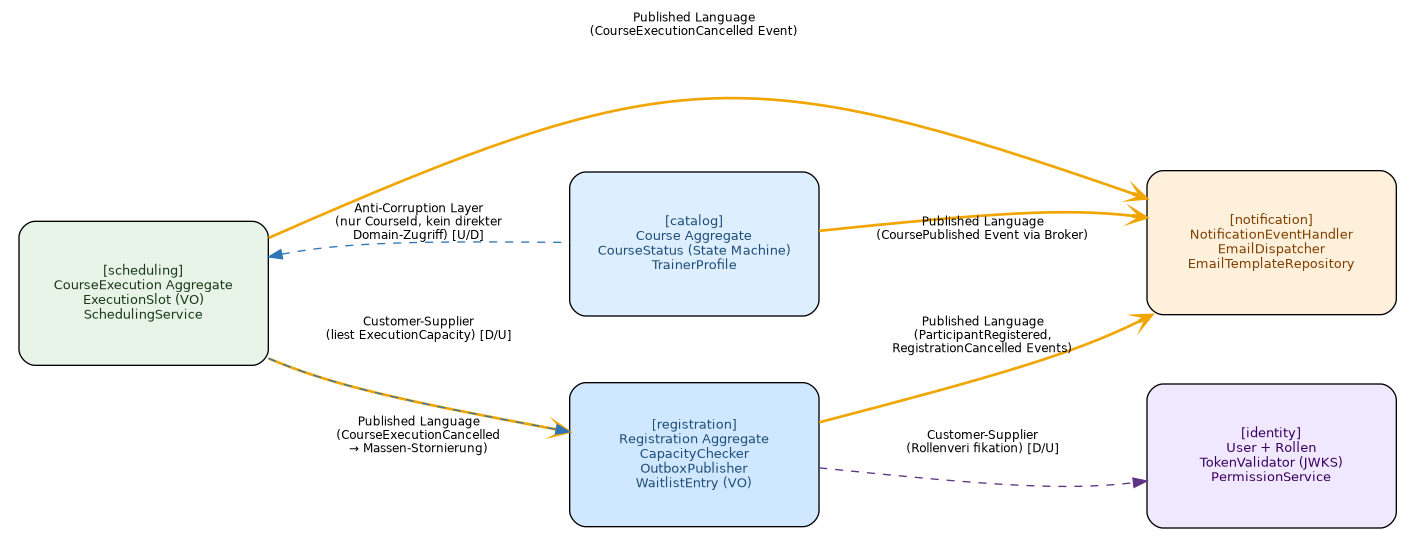
\includegraphics[width=\textwidth]{assets/context_map}
  \caption{\textit{DDD Context Map: Bounded Contexts und Beziehungen}}
  \label{fig:context_map}
\end{figure}

\begin{tabularx}{\textwidth}{L{3.5cm} L{3cm} X}
  \rowcolor{tableheader}
  \color{white}\textbf{Beziehung} &
  \color{white}\textbf{Muster (DDD)} &
  \color{white}\textbf{Erläuterung} \\

  scheduling $\leftrightarrow$ catalog &
  Anti-Corruption Layer\,(ACL) &
  Ein ACL ist eine Schutzschicht, die verhindert, dass
  das Domänenmodell eines fremden Contexts in den eigenen
  Code ``hineinwächst''. Konkret: \texttt{scheduling}
  übernimmt \emph{keine} Klassen oder Strukturen aus
  \texttt{catalog}, sondern übersetzt eingehende Daten
  an der Grenze in eigene Objekte. Es wird lediglich die
  \texttt{CourseId} als Referenz verwendet -- nie das
  vollständige Kursmodell. So bleibt \texttt{scheduling}
  unabhängig, selbst wenn sich das Modell in
  \texttt{catalog} ändert. \\

  \rowcolor{tablegrey}
  registration $\to$ scheduling &
  Customer-Supplier &
  In diesem Muster gibt es eine klare Rollenverteilung:
  Der \emph{Supplier} (Lieferant) stellt eine
  Schnittstelle bereit, der \emph{Customer} (Kunde)
  konsumiert sie. Hier liefert \texttt{scheduling} als
  Supplier Kapazitätsdaten (z.\,B.\ freie Plätze) über
  eine synchrone REST-API. \texttt{registration} als
  Customer ruft diese Daten ab, um bei einer
  Einschreibung zu prüfen, ob noch Plätze verfügbar
  sind. Der Supplier verpflichtet sich, die
  Schnittstelle stabil zu halten. \\

  registration $\to$ identity &
  Customer-Supplier &
  Gleiche Rollenverteilung: \texttt{identity} ist
  Supplier und stellt das Berechtigungsmodell bereit
  (Rollen, Berechtigungen). \texttt{registration} als
  Customer fragt bei Bedarf Rollendaten ab -- etwa um
  zu entscheiden, ob ein Nutzer eine Einschreibung
  stornieren darf. \\

  \rowcolor{tablegrey}
  catalog / reg / sched $\to$ notification &
  Published Language &
  Bei diesem Muster einigen sich die beteiligten Contexts
  auf ein \emph{gemeinsames, dokumentiertes Datenformat}
  für die Kommunikation -- hier in Form von Domain Events
  mit definierter JSON-Struktur (z.\,B.\
  \texttt{EnrollmentConfirmed}, \texttt{CoursePublished}).
  \texttt{notification} kennt \emph{aus\-schliess\-lich}
  dieses Event-Format und hat keinen Einblick in die
  internen Domänenmodelle der sendenden Contexts.
  Die Events werden asynchron über den Message Broker
  (RabbitMQ) transportiert. So kann
  \texttt{notification} eine Bestätigungsmail versenden,
  ohne zu wissen, wie eine Einschreibung intern
  modelliert ist. \\
\end{tabularx}

\subsubsection{Zusammenfassung der Architekturentscheidungen}

Die folgende Tabelle fasst die zentralen Architekturentscheidungen
zusammen, die aus der gewählten Microservice-Architektur und den
oben beschriebenen Bounded-Context-Beziehungen resultieren. Jede
Entscheidung ist in einem eigenen ADR (Kap.~9) ausführlich
dokumentiert und begründet.

\begin{tabularx}{\textwidth}{L{3.5cm} X L{2cm}}
  \rowcolor{tableheader}
  \color{white}\textbf{Entscheidung} &
  \color{white}\textbf{Begründung} &
  \color{white}\textbf{ADR} \\

  Microservices &
  Unabhängige Deployments, Team-Autonomie,
  horizontale Skalierung &
  ADR-001 \\

  \rowcolor{tablegrey}
  Database per Service &
  Verhindert Kopplung auf DB-Ebene; unabhängige
  Schema-Migrationen &
  ADR-001, ADR-006 \\

  REST + JSON &
  Standardprotokoll, breite Toolunterstützung &
  ADR-005 \\

  \rowcolor{tablegrey}
  Asynchrones Messaging &
  Entkopplung; Resilienz bei Teilausfällen &
  ADR-002 \\

  Transactional Outbox &
  Atomare Event-Persistenz; verhindert
  Dual-Write-Problem &
  ADR-004, ADR-009 \\

  \rowcolor{tablegrey}
  Container / Kubernetes &
  Einheitliches Deployment, Auto-Scaling,
  Cloud-Portabilität &
  ADR-001 \\

  Externer OIDC-IdP &
  Security-Best-Practices, MFA,
  DSGVO-Compliance &
  ADR-003 \\

  \rowcolor{tablegrey}
  Angular / Vue.js SPA &
  Reaktive UX; bekanntes Ökosystem im Team &
  ADR-005 \\
\end{tabularx}


% ──────────────────────────────────────────────
\subsection{Übergreifende Architekturprinzipien}

Die folgenden Prinzipien sind die nicht-verhandelbaren Leitlinien
der EduPlanner-Architektur. Sie gelten serviceübergreifend und
dienen als Entscheidungsrahmen im Entwicklungsalltag: Wann immer
eine Design-Frage aufkommt, geben diese Prinzipien die Richtung
vor. Einzelne Architekturentscheidungen (Kap.~9) lassen sich
jeweils auf eines oder mehrere dieser Prinzipien zurückführen.

\begin{itemize}[leftmargin=1.5em]
  \item \textbf{Favour Async over Sync:}
  Zustandsändernde Operationen zwischen Bounded Contexts
  erfolgen ausschliesslich via Domain Events. Synchrone
  REST-Aufrufe nur für lesende Operationen.
  \item \textbf{No Shared Databases:}
  Kein direkter Cross-Service-Datenbankzugriff.
  \item \textbf{Fail Fast, Recover Gracefully:}
  Transiente Fehler durch Retry + Exponential Backoff.
  Nicht-kritische Ausfälle (z.\,B.\ \texttt{notification})
  blockieren nie den Kernprozess.
  \item \textbf{Security by Default:}
  JSON-Web-Token-Validierung (JWT) am Gateway;
  zusätzliche rollenbasierte Zugriffskontrolle
  (Role-Based Access Control, RBAC) in jedem Service.
  \item \textbf{Privacy by Design:}
  Keine personenbezogenen Daten (Personally Identifiable
  Information, PII) in Logs, Events oder Metriken. Events
  referenzieren ausschliesslich \texttt{userId}, nie
  E-Mail-Adresse oder Name.
  \item \textbf{Explizite Architekturentscheidungen:}
  Jede signifikante Entscheidung wird als Architecture
  Decision Record (ADR) dokumentiert.
\end{itemize}


% ──────────────────────────────────────────────
\subsection{Qualitätsziel-Mapping}

Jede Architekturentscheidung in EduPlanner dient mindestens einem
übergeordneten Qualitätsziel. Die folgende Tabelle macht diesen
Zusammenhang explizit: Sie ordnet den zentralen Qualitätszielen
nach ISO~25010\footnotemark{} die jeweils wichtigsten
Architekturmassnahmen zu. So wird nachvollziehbar, \emph{warum}
bestimmte Muster und Technologien gewählt wurden -- und welche
Kapitel die jeweilige Massnahme im Detail beschreiben.

\footnotetext{%
  \textbf{ISO~25010} ist ein internationaler Standard, der ein
  Qualitätsmodell für Softwareprodukte definiert. Er gliedert
  Qualität in acht Hauptmerkmale -- darunter Funktionalität,
  Zuverlässigkeit, Sicherheit, Wartbarkeit und Benutzbarkeit.
  Das Modell dient als gemeinsame Sprache, um Qualitätsanforderungen
  messbar und vergleichbar zu formulieren.%
}

\begin{tabularx}{\textwidth}{L{4cm} X L{2cm}}
  \rowcolor{tableheader}
  \color{white}\textbf{Qualitätsziel (ISO~25010)} &
  \color{white}\textbf{Architekturmassnahme} &
  \color{white}\textbf{Referenz} \\

  Functional Correctness &
  \emph{Optimistic Locking} stellt sicher, dass parallele
  Änderungen an denselben Daten (z.\,B.\ zwei gleichzeitige
  Einschreibungen auf den letzten Platz) erkannt und
  konfliktfrei aufgelöst werden. Alle Schreiboperationen
  erfolgen transaktional. Event-Handler sind
  \emph{idempotent} -- d.\,h.\ ein mehrfach empfangenes
  Event führt nicht zu doppelten Einschreibungen. &
  Kap.~5.4, 8.4 \\

  \rowcolor{tablegrey}
  Reliability -- Availability &
  Kubernetes \emph{Health-Probes} (Liveness / Readiness)
  erkennen ausgefallene Pods und starten sie automatisch
  neu. \emph{Circuit Breaker} (via Resilience4j) verhindern,
  dass der Ausfall eines Services sich kaskadenartig auf
  andere ausbreitet. Die PostgreSQL-Datenbanken laufen
  redundant; der Message Broker (RabbitMQ) wird als Cluster
  betrieben. &
  Kap.~8.2, 7.4 \\

  Maintainability &
  Die strikten Bounded-Context-Grenzen sorgen dafür, dass
  Änderungen an einem Service keine Seiteneffekte in
  anderen Services verursachen. Kein Service greift direkt
  auf die Datenbank eines anderen zu. Alle architekturrelevanten
  Entscheidungen sind in ADRs (Kap.~9) festgehalten, sodass
  das Projektteam auch Monate später nachvollziehen kann,
  \emph{warum} etwas so entschieden wurde. &
  Kap.~5, 9 \\

  \rowcolor{tablegrey}
  Security &
  JSON Web Tokens (JWT) werden am API-Gateway validiert;
  jeder Service führt zusätzlich eine eigene rollenbasierte
  Zugriffskontrolle (RBAC) durch. Sämtliche Kommunikation
  läuft über HTTPS/TLS. In Logs, Events und Metriken werden
  keine personenbezogenen Daten (PII) gespeichert. &
  Kap.~8.1, 8.2 \\

  Usability &
  Die Single-Page-Application (Angular oder Vue.js) bietet
  eine reaktive Benutzeroberfläche ohne Seitenwechsel.
  Formulare sind auf minimale Eingaben optimiert.
  \emph{Progressive Loading} lädt nur die aktuell benötigten
  Inhalte nach, um die wahrgenommene Ladezeit zu reduzieren.
  Der Mobile-First-Ansatz stellt sicher, dass das Interface
  auch auf Smartphones nutzbar ist. &
  ADR-005 \\
\end{tabularx}

% ──────────────────────────────────────────────
\subsection{Skalierungsstrategie pro Bounded Context}

Nicht alle Services von EduPlanner sind gleich stark belastet.
Der \texttt{registration}-Service erlebt beispielsweise zu
Einschreibungsfristen hohe Lastspitzen, während \texttt{catalog}
überwiegend Lesezugriffe bedient. Deshalb wird jeder Service
individuell skaliert.

Die Skalierung erfolgt automatisiert über den Kubernetes
\emph{Horizontal Pod Autoscaler} (HPA): Sobald ein definierter
Schwellenwert (\emph{Scale-Trigger}) überschritten wird, startet
Kubernetes zusätzliche Pod-Instanzen des betroffenen Services --
bis zur konfigurierten Obergrenze. Fällt die Last wieder, werden
überschüssige Pods abgebaut. Die Spalten \emph{Min~Pods} und
\emph{Max~Pods} definieren den Skalierungskorridor pro Service.

\begin{tabularx}{\textwidth}{L{3cm} C{2cm} C{2cm} X}
  \rowcolor{tableheader}
  \color{white}\textbf{Service} &
  \color{white}\textbf{Min~Pods} &
  \color{white}\textbf{Max~Pods} &
  \color{white}\textbf{Scale-Trigger} \\

  registration & 2 & 10 &
  CPU-Auslastung $>$ 70\,\% oder
  Warteschlangentiefe $>$ 100~Nachrichten \\

  \rowcolor{tablegrey}
  catalog & 1 & 3 &
  CPU-Auslastung $>$ 80\,\%
  (primär Lesezugriffe) \\

  scheduling & 2 & 5 &
  CPU-Auslastung $>$ 70\,\% \\

  \rowcolor{tablegrey}
  notification & 1 & 10 &
  Warteschlangentiefe $>$ 500~Nachrichten \\

  identity & 2 & 5 &
  Antwortzeit (Request-Latency) $>$ 200\,ms \\
\end{tabularx}
